%!TEX root = ../Report.tex

In this chapter, we cover the overall design of the project, leaving the details of the systems produced for chapter \ref{chapter:implementation}, which covers the implementation. We first describe the aim of this project, and our goals for this year. Next, we present the corresponding high level plan. Finally, we give the design of some additional experiments which will provide further insights into the questions posed in this project.



\section{Project Goal}
\label{section:design:project_goal}

The main goal of this project is to investigate if we can gain some extra performance in parallel multi-programming systems by exploiting contention aware scheduling and plastic programming. In the previous year, we investigated the design and performance of a complete plastic parallel programming library, and created some prototype software for such a system. The conclusion was that such a system would be viable, as the overhead introduced was minimal. 

This year, our focus will be on what, if any, performance we can gain from the use of such a system. Therefore, we do not need to design and implement a complete programming library, (as was done in the previous year), we just need some stripped down software which would let us carry out our plastic performance experiments. Packaging this into a complete system could be future work, this is discussed further in section \ref{section:conclusion_and_future_work:future_work}.



\section{Project Architecture}
\label{section:design:project_archetecture}

Here we present an itemised list of steps, established at the start of this year of the project, which form the high level plan of how we will achieve our aim. We go on to expand upon each point with explanations and justifications for the choices made.

\begin{enumerate}
    \item Select parallel pattern
    
    \item Investigate performance characteristics
    
    \item Find interesting instances of pattern
    
    \item Perform refined investigation of interesting instances
    
    \item Perform contention aware plasticity analysis
\end{enumerate}



\subsection{Parallel Pattern Selection}
\label{section:design:parallel_pattern_selection}

In the previous year, we focused on the map-array parallel pattern. This pattern is fairly predictable in terms of complexity and performance characteristics, in that providing more cores and corresponding threads to the computation will generally improve performance. Because of this, each program will effectively be able to saturate all the cores allocated to it. This is the ideal for any efficiency focused application, and as a result we have little room for improvement. Therefore, this year, we decided to focus on a more interesting parallel pattern which would not necessarily improve with extra cores.

There are many options for us to choose from \cite{parallel_patterns_examples1} \cite{parallel_patterns_examples2}, which could be explored in future research, including pipelines, recursive splitting, and geometric decomposition. Ideally, we want a pattern which is widely used in real applications, providing interesting use cases, and possessing less predictable performance characteristics than map-array. Accordingly, we selected stencil codes as the parallel pattern to focus on.

Stencil codes are a class of iterative kernels which update the elements of an array, (we refer to this as the data grid), according to some fixed pattern, called a stencil. Typically, after one pass of the array, some sort of convergence test is run to check if the computation is complete. Stencil codes are used in computational fluid dynamics, in linear algebra for solving partial differential equations \cite{yang_mittal_2014} \cite{anzt_dongarra_quintana-ort_2015} \cite{wang_2015}, in image processing, and in cellular automata. In general, many algorithms which operate on finite grids can be formulated as a stencil code.
 
Stencil codes should have more interesting performance characteristics since they have inherent data sharing properties. The data grid is divided between threads, and when a thread updates a particular point in the grid, it will access the neighbours of that point, and those neighbours may be in a portion of the grid associated with another thread.
 
For selecting interesting instances, we can vary the size of the data grid, the computation performed at each point, and the number of iterations (passes over the array) before the computation is complete. In a real application, the number of iterations would vary, however we want a reproducible, predictable instance. To this end, we simulate convergence tests, and manually end the computation after N iterations.



\subsection{Performance Characteristics Investigation}
\label{section:design:performance_characteristics_investigation}

The intention behind this part of the project is to get a feel for the performance characteristics of our chosen parallel pattern. To do this, we need to create an implementation of the parallel pattern, and generate a synthetic problem to run our pattern on. We add the ability to vary characteristics of both the problem and the implementation, allowing us to perform this basic investigation. In particular, we would like to vary the following parameters:

Problem parameters
\begin{itemize}
    \item Grid size
    \item Computation kernel
    \item Number of iterations
\end{itemize}

Implementation parameters
\begin{itemize}
    \item Number of workers
    \item Thread pinnings
\end{itemize}



A synthetic stencil with these features would give us a good starting point, and enable us to perform our experiments. From here, we can begin to explore the performance characteristics of such a stencil.

Between iterations, stencil codes use a barrier, in order to synchronise threads. An interesting experiment would be to investigate what effect this has on performance, since it requires communication and synchronisation between threads. The cost of this operation is dependent upon the number of threads, and the work that they do, both aspects of the program we wish to vary for later experiments. This is the first of the two experiments we plan for the performance characteristics investigation.

Another mechanism which stencil codes use between iterations is some sort of convergence test. A convergence test essentially is a test for whether a computation is complete. After a successful test, we end the computation. Similar to barriers, they require communication and synchronisation between threads, making their performance impact variable. Unlike barriers however, they are not always essential to the computation, and are application dependent. An investigation into the impact of the convergence test would be a valuable insight. This is the second of the two experiments we plan for the performance characteristics investigation.

Here, we discuss a prediction of how the stencil codes will behave. An artefact of a large grid size is that it is less likely that threads would interfere, as the border between their section of data and their neighbours has the same size. Their overall area has increased however, making it less likely that two threads are on their respective borders simultaneously. This is illustrated in figure \ref{fig:grid_comparison}.



\begin{figure}[ph]
    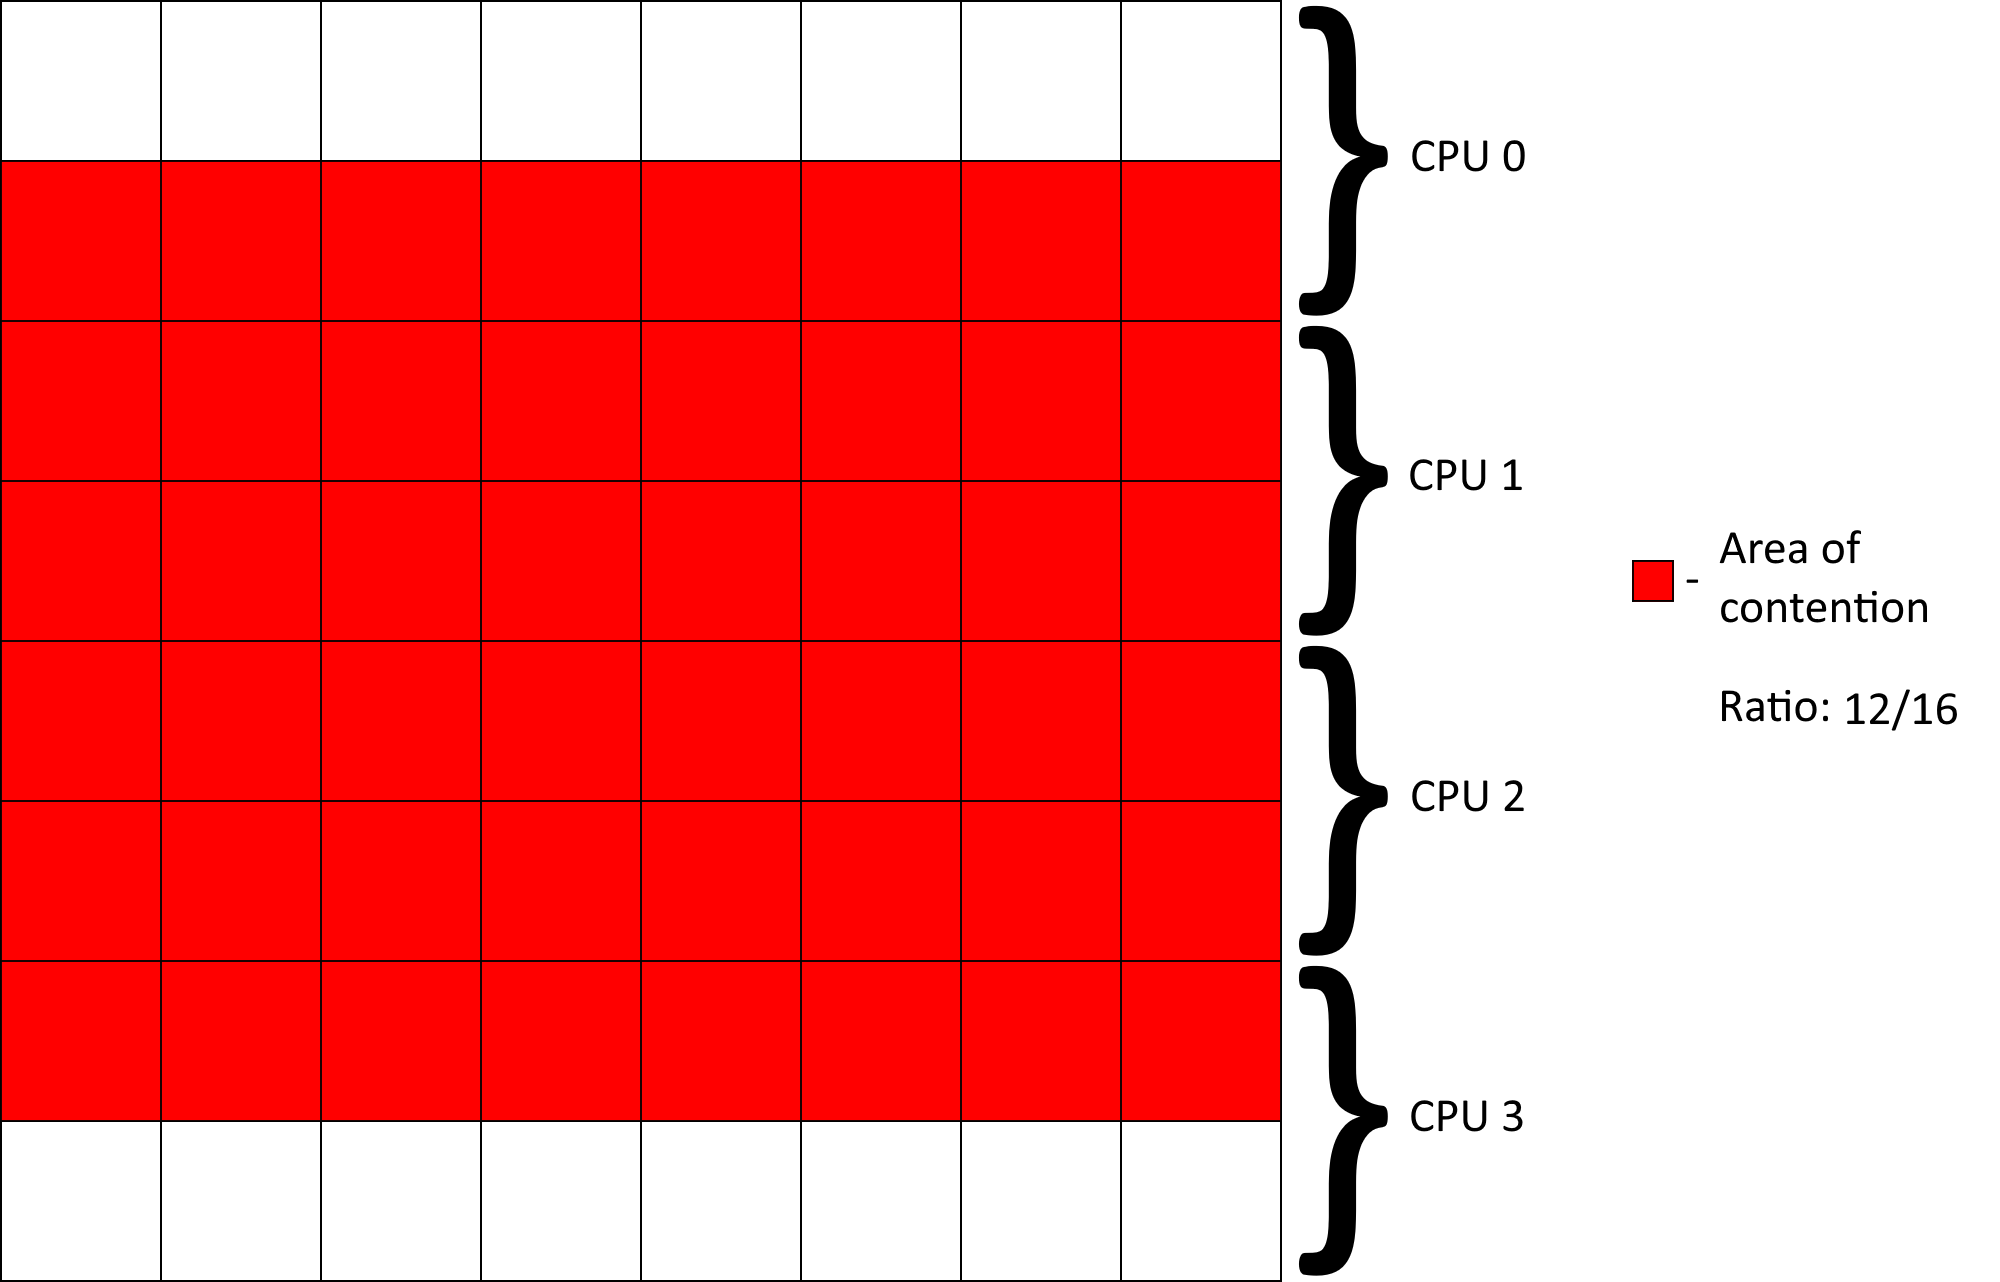
\includegraphics[width=1\textwidth]{graphics/8_with_info.png}
    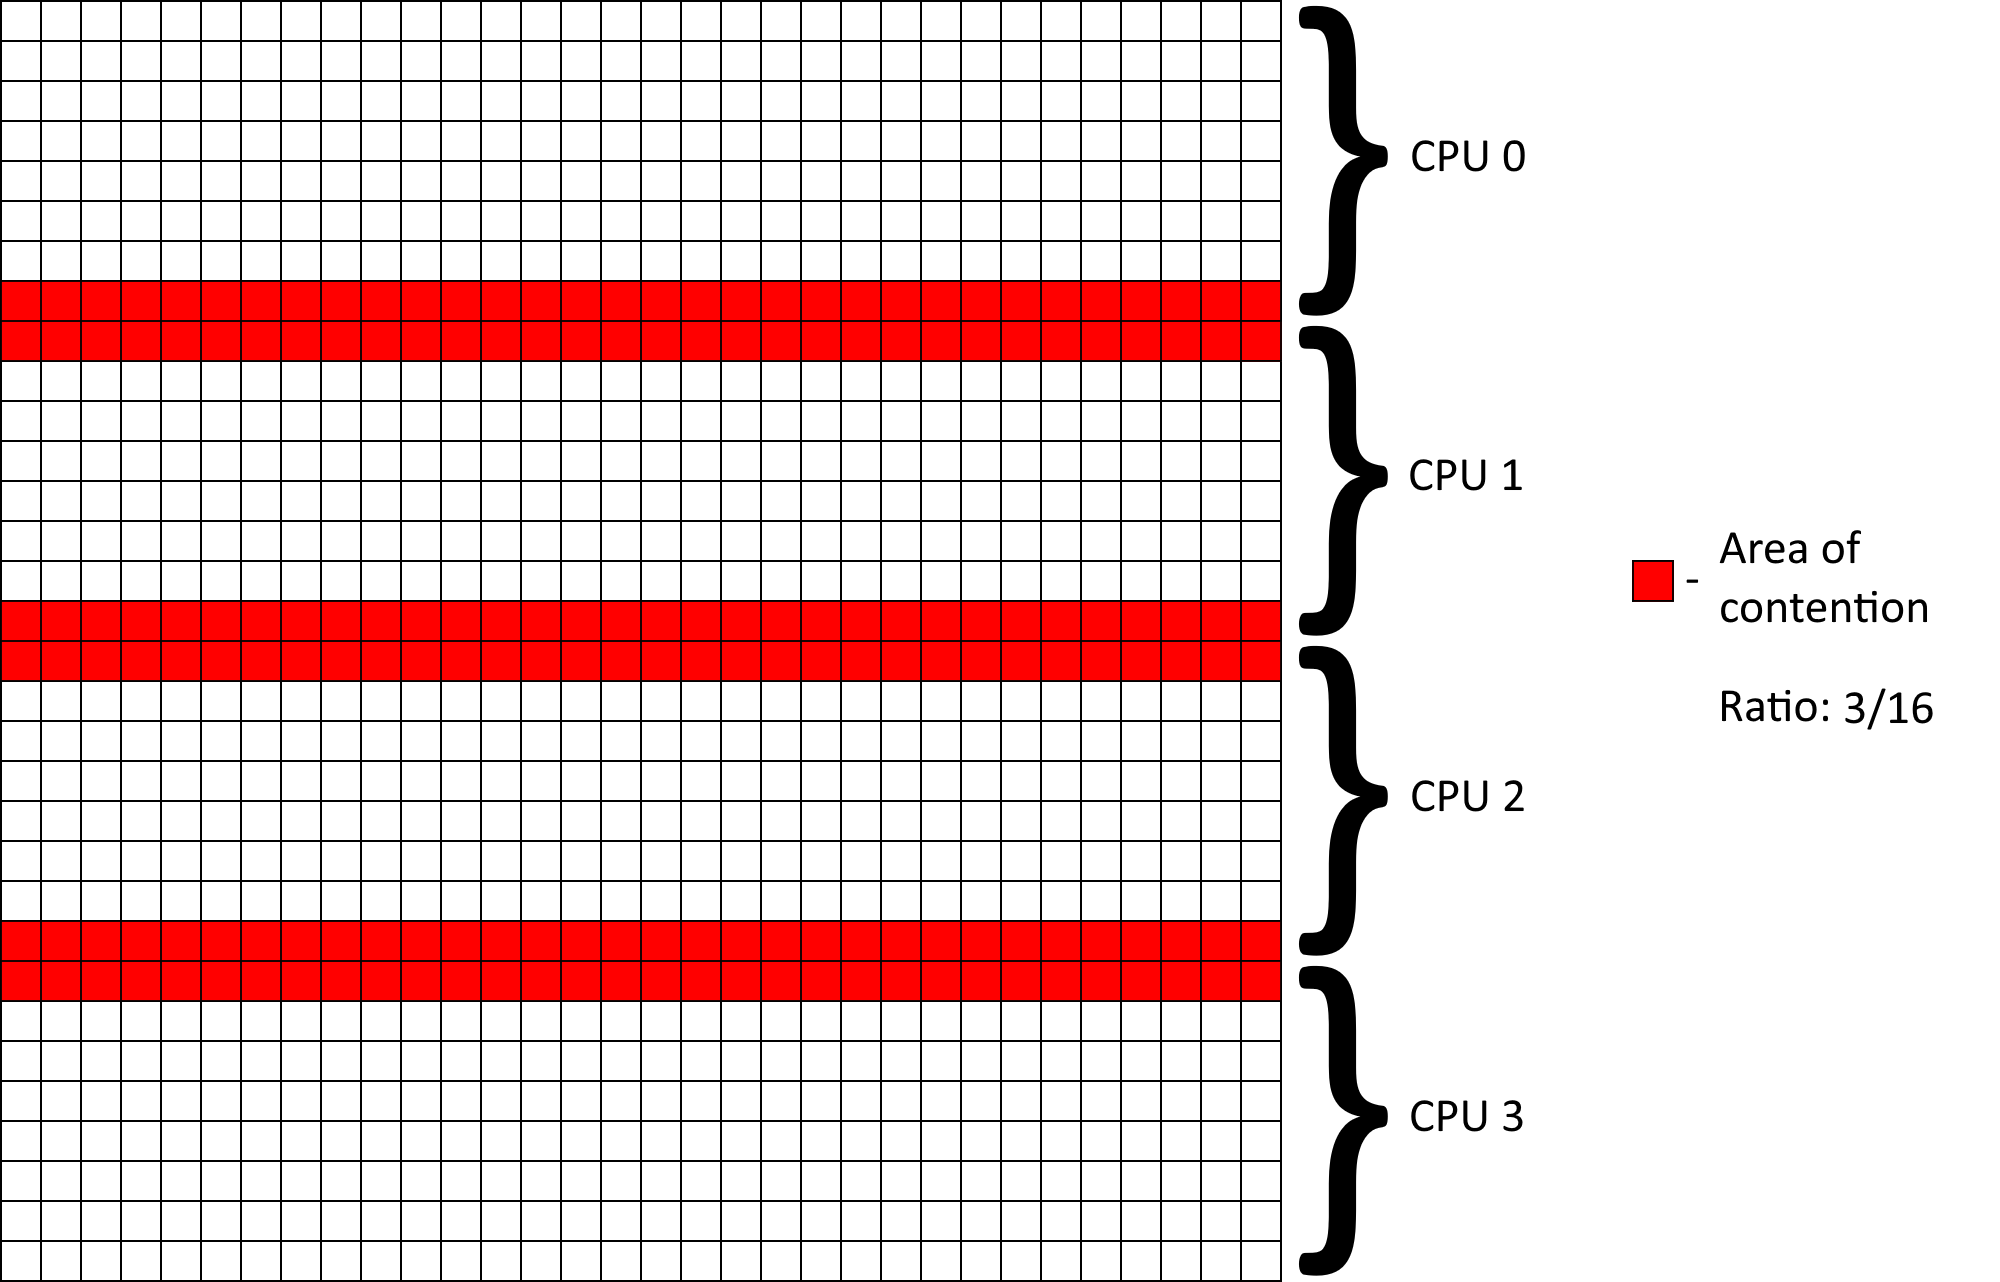
\includegraphics[width=1\textwidth]{graphics/32_with_info.png}
    \caption{A visualisation of how the areas of contention change when we increase the gridsize. Different threads can only encounter contention along the edges of their designated area, so as we increase the size of the grid, the ratio of area where a thread may experience contention compared to the area where it cannot shinks.}
    \label{fig:grid_comparison}
\end{figure}



Comparably, with a more complex, time consuming kernel, threads are less likely to interfere, for similar reasons. Instead of being more distant in space, they are more distant in time, making it less likely that two threads are on their respective borders simultaneously. 

The point of all this is that the interference between threads should decrease as the grid size or kernel complexity increases, and as such, we should expect better scaling of performance with large grid sizes and complex kernels. This is not only because of the reduced interference, but also because the proportion of useful work to overhead is larger, meaning that the overhead costs can be more easily hidden.



\subsection{Finding Interesting Instances}
\label{section:design:interesting_instances}

In this section, and in this report as a whole, when we discuss performance curves, we refer to the curve on a graph of the runtime of an instance, against the number of threads used. Examples of real performance curves can be seen in section \ref{section:results:performance_characteristics_investigation}, with figures \ref{fig:barrier_sync} and \ref{fig:convergence_checks}.

In selecting interesting instances, we want to find instances with different characteristic performance curves, and some instances which utilise different resources. The rationale behind this is that they should make valuable test cases for our contention aware plasticity experiments. The differing performance curves may mean that the partitioning of resources is asymmetrical, and the differing resource utilisation may mean that these programs work well together, i.e. they have less contention since they require different resources.

This section will be informed by the results of the previous one, the performance characteristics investigation. We are hoping that by varying the total amount of work to be done, (grid size and computation kernel complexity), we can produce at least two distinct performance curves; one with a small amount of work, meaning parallelisation overhead will be more significant, so more threads may not necessarily be a good thing, and one with a large amount of work, which can always use more threads than we have.

In addition to varying the work size, we can change the computation kernel to utilise different resources, e.g. CPU and RAM. This will give us at least two more instances per resource. 

Finally, if time allows, we could produce additional instances by adding a random component to the computation kernel. Many stencils do not have an equally distributed amount of work across the grid. Randomising the amount of work to be done at each point in the grid models this situation. This will double our number of instances, one with a random component, and one without, and as such, it may result in an impractical number of experiments.

There is a motivation for keeping our number of test instances down, and in fact a reason why we cannot exhaustively test every instance. Each instance will require a significant amount of experiments, which could take hours or even days. Increasing the number of test cases will greatly increase the number of combinations of pairs for the pairwise contention aware plasticity experiments. Just finding the optimal number of threads for a given number of CPU cores requires $(C + T) * C$ experiments, where $C$ is the number of cores, and $T$ is how much we ``overshoot'' the number of cores. We do this because we may gain some interesting results from having more threads than cores.



\subsection{Finding Optimal Thread Counts}
\label{section:design:optimal_threads}

Here we will perform a refined investigation of each chosen instance. The aim is to establish the performance characteristics of each interesting instance we find, such that they can be used as a baseline for comparison (one of the program running in isolation). In previous experiments, we were interested in the features of the stencil code itself, (e.g. barrier synchronisation), however now we are interested in the overall performance, and since performance may vary from machine to machine, we will repeat each experiment on a variety of machines, to give us a comparison.

To reduce the complexity of our experiments, we will restrict our implementation parameters to just the number of workers and what CPU cores they are pinned to. Again, since our experiments will be so time intensive, to reduce complexity we will focus on finding the optimal number of threads for every possible given number of provided CPU cores. Each thread will have access to any of the cores provided, meaning that this is akin to just limiting the CPU cores of a program, and as such this represents a typical implementation without any plasticity or contention aware scheduling, giving us the baseline performance.



\subsection{Contention Experiments}
\label{section:design:contention_experiments}

In order to test if extending contention aware scheduling with plasticity is worth it, we need to experiment with programs running simultaneously, on a real multiprogramming system. We will focus on two programs running simultaneously, to keep the number of possible combinations in the parameter space practical. 

With two programs, we have four parameters, that is, the number of workers and the number of CPU cores assigned to each program. We wish to test the performance of each program when run simultaneously for each combination of these parameters, in order to find the optimal configuration. Taking the results of the previous experiment into account (where we should find the best parameters for each program in isolation), we can investigate the performance of the configuration where we use these parameters. The difference between this value and the value given by the optimal configuration will tell us if we can gain any performance from contention aware scheduling, completing the main goal of this project.

So that we can compare our results to the previous experiment, again each thread will have access to any of the cores provided. Both programs will start simultaneously, and we will measure overall performance in terms of throughput, by summing the runtime of each program. Also as with the previous experiment, we will endeavour to run these experiments across multiple machines.

The size of the parameter space of two programs running simultaneously is $O(N^4)$ where $N$ is the number of options for each parameter. This is because both programs have two parameters which can be varied, which are the number of cores to use, and the number of threads to use. Exhaustively testing this space is likely to be unrealistic due to time constraints, therefore, we may need to reduce the number of experiments as time allows. This will be discussed further in chapter \ref{chapter:experimental_methodology}.



\section{Additional Experiments}
\label{section:design:additional_experiments}

With the above set of experiments, we will have answered the main question posed for this project. That is, can we gain any significant performance by utilising both contention aware scheduling and plastic parallel programming. In this section, we present some additional experiments which should provide some further insight into the system, which were designed and performed later as time allowed.



\subsection{Extended Contention Experiments}
\label{section:design:extended_contention_experiments}

We build upon our contention experiments by performing additional ones with three programs running in contention. This provides an interesting insight to a more complex scenario. However, with three programs, we have six parameters to vary, (the number of threads and the number of cores assigned to each program). With six parameters, the size of the parameter space is $O(N^6)$, where as above, $N$ is the number of options for each parameter. Because of this, we have to drastically reduce the number of tests that we perform.



\subsection{Plastic Experiments}
\label{section:design:plastic_experiment}

With our contention experiments, will have hopefully demonstrated that there is potential for clear, tangible gain to be had with our system. We intended to further this by demonstrating our system plastically switching implementations, and showing an improvement in the runtime. 

To carry this out, we would select one of our contention experiments, and design an experiment where our program initialises with a sub-optimal configuration, and subsequently plastically changes to the optimal configuration. We would then compare this to the case where we did not plastically change.

We designed and programmed this experiment, however, unfortunately we did not have the time to run it.